% ============================================================
%  CSC8851 Spring 2026 — Preliminary Project Report
%  Author : Bryan Chau, Katelyn Truong, Loc Giang
%  Format : IEEE CVPR 2-column (10pt, letterpaper)
% ============================================================
\documentclass[10pt,twocolumn,letterpaper]{article}

% ── Page geometry ────────────────────────────────────────────
\usepackage[
  top=1in,
  bottom=1in,
  left=0.75in,
  right=0.75in,
  columnsep=0.25in
]{geometry}

% ── Typography & encoding ────────────────────────────────────
\usepackage[T1]{fontenc}
\usepackage[utf8]{inputenc}
\usepackage{times}           % Times New Roman (IEEE standard)
\usepackage{microtype}

% ── Math ─────────────────────────────────────────────────────
\usepackage{amsmath, amssymb, bm}

% ── Figures & tables ─────────────────────────────────────────
\usepackage{graphicx}
\usepackage{booktabs}
\usepackage{multirow}
\usepackage{caption}
\usepackage{subcaption}
\usepackage[table]{xcolor}
\usepackage{tikz}
\usetikzlibrary{shapes.geometric, arrows.meta, positioning, fit, backgrounds}

% ── URLs & hyperlinks ────────────────────────────────────────
\usepackage[hidelinks]{hyperref}
\usepackage{url}

% ── Section title spacing ────────────────────────────────────
\usepackage{titlesec}
\titlespacing*{\section}{0pt}{8pt plus 2pt minus 2pt}{4pt plus 1pt}
\titlespacing*{\subsection}{0pt}{6pt plus 2pt}{2pt plus 1pt}

% ── Paragraph spacing ────────────────────────────────────────
\setlength{\parskip}{2pt}
\setlength{\parindent}{1em}

% ── Header / footer ──────────────────────────────────────────
\usepackage{fancyhdr}
\pagestyle{fancy}
\fancyhf{}
\renewcommand{\headrulewidth}{0pt}
\fancyfoot[C]{\thepage}

% ── Algorithm ────────────────────────────────────────────────
\usepackage{algorithm}
\usepackage{algpseudocode}

% ── Convenient shorthands ────────────────────────────────────
\newcommand{\eg}{\textit{e.g.},\xspace}
\newcommand{\ie}{\textit{i.e.},\xspace}
\newcommand{\etal}{\textit{et al.}\xspace}
\newcommand{\wrt}{w.r.t.\xspace}
\usepackage{xspace}

% ── Caption style ────────────────────────────────────────────
\captionsetup{font=small, labelfont=bf, skip=4pt}

% ─────────────────────────────────────────────────────────────
\begin{document}

% ── Title block ──────────────────────────────────────────────
\title{%
  \vspace{-0.4cm}
  {\large\textbf{Food Nutrition Estimation from a Single RGB Image:\\
  A Weight-First Pipeline with Geometric Feature Extraction}}%
  \vspace{-0.2cm}
}

\author{%
  \begin{tabular}{ccc}
    \begin{minipage}{0.31\linewidth}\centering\small
      \textbf{Bryan Chau}\\[2pt]
      \texttt{nchau1@student.gsu.edu}\\[2pt]
      \textbf{PantherID: 002508179}
    \end{minipage} &
    \begin{minipage}{0.31\linewidth}\centering\small
      \textbf{Loc Giang}\\[2pt]
      \texttt{lgiang2@student.gsu.edu}\\[2pt]
      \textbf{PantherID: 002505346}
    \end{minipage} &
    \begin{minipage}{0.31\linewidth}\centering\small
      \textbf{Katelyn Truong}\\[2pt]
      \texttt{ltruong18@student.gsu.edu}\\[2pt]
      \textbf{PantherID: 002852993}
    \end{minipage} \\
  \end{tabular}
}

\date{}
\maketitle
\thispagestyle{fancy}

% ── Abstract ─────────────────────────────────────────────────
\begin{abstract}
Accurate nutritional estimation from food photographs has broad applications in
dietary monitoring and public health, yet remains challenging due to the
diversity of portion sizes, food types, and imaging conditions.  We present a
multi-stage deep learning pipeline that estimates calories, fat, protein, and
carbohydrates from a single RGB image.  The system first segments the food
region with YOLOv8-seg, estimates relative depth with MiDaS, and extracts nine
geometric features encoding plate coverage and food volume.  A lightweight
4-layer MLP (WeightMLP) then predicts dish weight in grams; macros are derived
by multiplying the predicted weight by per-nutrient density constants computed
from the Nutrition5K dataset.  A food-type classifier (EfficientNet-B0
fine-tuned on Food-101) triggers per-food density lookup from the USDA
FoodData Central API, replacing global constants when a match is found.  MC
Dropout propagates uncertainty through all stages.  On the Nutrition5K test
split ($n{=}325$), the weight-first pipeline achieves a calorie MAE of
approximately \textbf{119.8 kcal} and an RMSE of \textbf{158.7 kcal}, with
the ensemble reducing variance relative to each standalone stage.  A live
Gradio demo allows upload of arbitrary food photos and displays per-food
calorie breakdowns with uncertainty intervals.
\end{abstract}

% ─────────────────────────────────────────────────────────────
\section{Introduction}
\label{sec:intro}
% ─────────────────────────────────────────────────────────────

Dietary tracking is a cornerstone of managing chronic disease, athletic
performance, and weight control.  Manual food logging is burdensome and prone
to systematic underreporting~\cite{dhurandhar2015}; an automatic vision-based
estimator that operates from a simple photograph could remove this friction
entirely.  The problem is non-trivial: two dishes that look geometrically
similar (\eg,\, a bowl of ramen vs.\ a bowl of salad) carry vastly different
caloric loads, while the same food photographed at different distances or
viewing angles yields wildly varying apparent sizes.

\paragraph{Challenge statement.}
Given a single uncalibrated RGB image $\mathbf{I} \in \mathbb{R}^{H \times W
\times 3}$, produce predictions
\begin{equation}
  \hat{\mathbf{n}} = \bigl(\hat{n}_{\text{cal}},\;
                           \hat{n}_{\text{fat}},\;
                           \hat{n}_{\text{pro}},\;
                           \hat{n}_{\text{carb}}\bigr)
  \label{eq:problem}
\end{equation}
where each quantity is in kilocalories or grams respectively, along with a
calibrated uncertainty estimate $\hat{\boldsymbol{\sigma}}$.

\paragraph{Key insight.}
We decouple the estimation into two sub-problems.  First, predict dish
\emph{weight} $\hat{w}$ from purely physical (geometric) signals — food mask
area and depth statistics — which is a dimensionality reduction from raw pixels
to a scalar with clear physical meaning.  Second, multiply by food-class
density constants to recover macros:
\begin{equation}
  \hat{n}_k = \hat{w} \cdot \bar{c}_k,
  \qquad k \in \{\text{cal, fat, pro, carb}\}.
  \label{eq:weight_first}
\end{equation}
This separation is more interpretable and more easily improved (better density
constants from a larger food database) than end-to-end calorie regression.

\paragraph{Scope of this report.}
This preliminary report documents the motivation, related literature, and
complete system design.  Quantitative results on the Nutrition5K test split are
reported where training has been completed; placeholder figures are included for
experiments still in progress.

% ─────────────────────────────────────────────────────────────
\section{Related Work}
\label{sec:related}
% ─────────────────────────────────────────────────────────────

\subsection{Food Recognition}

Deep convolutional networks dominate food-image classification.  Bossard~\etal
\cite{bossard2014food101} introduced Food-101, a benchmark of 101\,000 images
across 101 categories, and reported $56.4\%$ top-1 accuracy with
\textit{Random Forests on CNN features}; subsequent fine-tuning of VGGNet and
ResNet architectures pushed accuracy above 85\%.  EfficientNet~\cite{tan2019efficientnet},
the backbone we adopt for food-type classification, achieves state-of-the-art
accuracy at an order-of-magnitude lower parameter count than VGG/ResNet through
compound coefficient scaling of depth, width, and resolution.  More recently,
Vision Transformers (ViTs)~\cite{dosovitskiy2020vit} and CLIP~\cite{clip2021}
have been applied to zero-shot food recognition, but their compute requirements
make them impractical for the lightweight real-time demo we target.

\subsection{Portion-Size Estimation and Depth}

Accurate calorie prediction requires estimating \emph{how much} food is present,
not only what it is.  Early approaches relied on calibration objects (\eg,\, a
known-size marker on the plate)~\cite{dehais2017}.  Later systems used stereo
RGB-D cameras; the Nutrition5K dataset~\cite{thames2021nutrition5k} collected
overhead RGBD images of cafeteria dishes with ground-truth macro labels,
enabling supervised learning of geometric features directly.  Monocular depth
estimation removes the need for specialised hardware.  MiDaS~\cite{ranftl2020midas}
provides robust relative depth from a single RGB image by training on multiple
datasets with mixed-scale supervision; we use the lightweight
\textit{MiDaS-small} variant for efficiency.

\subsection{Food Volume and Nutrition Estimation}

He~\etal~\cite{he2021nutritionfromimage} combine 3-D food reconstruction with a
food-ingredient database for calorie estimation, achieving MAEs of roughly
$100$--$150\,\text{kcal}$ on controlled benchmarks.  The NutriNet
system~\cite{ciocca2017nutrinet} uses 2-D image features with a nutrition
knowledge graph.  INGR-360~\cite{ingred360} estimates ingredient quantities from
360° photos.  Compared with these systems, our approach is designed to run on
consumer hardware (CPU) without depth sensors or food databases requiring manual
curation, relying only on freely available USDA FoodData Central for density
constants.

\subsection{Uncertainty Quantification in Neural Networks}

MC Dropout~\cite{gal2016mcdropout} approximates Bayesian inference by sampling
$T$ forward passes with dropout active at test time.  The sample mean and
standard deviation provide a lightweight uncertainty estimate without additional
parameters.  For regression tasks with uncertainty that propagates linearly through a
multiplication ($\hat{n}_k = \hat{w} \cdot \bar{c}_k$, Eq.~\ref{eq:weight_first}),
the macro uncertainty is simply
$\hat{\sigma}_{n_k} = \hat{\sigma}_w \cdot \bar{c}_k$,
where $\hat{\sigma}_w$ is the MC Dropout standard deviation of the weight
prediction.  Deep Ensembles~\cite{lakshminarayanan2017ensembles} offer stronger
calibration but at higher cost; we approximate ensemble diversity by combining
the weight-first stage (Phase~6) with the direct regression stage (Phase~4).

\subsection{Object Detection and Segmentation}

YOLOv8-seg~\cite{yolov8} extends the single-stage YOLO object detection
framework with an additional segmentation head, producing polygon masks at
real-time speeds.  We use the segmentation masks to isolate the food region from
the background before extracting depth statistics, substantially reducing noise
from non-food depth values (plates, cutlery, table surface).

% ─────────────────────────────────────────────────────────────
\section{Dataset}
\label{sec:dataset}
% ─────────────────────────────────────────────────────────────

\paragraph{Nutrition5K~\cite{thames2021nutrition5k}.}
Our primary training dataset consists of 3{,}247 overhead RGBD images of
Google cafeteria dishes.  Each dish is annotated with ground-truth mass (grams),
calories (kcal), fat (g), protein (g), and carbohydrates (g).  Images are
captured with a RealSense D415 camera at a fixed overhead angle under controlled
lighting.  Summary statistics are given in Table~\ref{tab:dataset}.

\begin{table}[h]
  \centering
  \caption{Nutrition5K dataset statistics (valid dishes, $n{=}3247$).}
  \label{tab:dataset}
  \setlength{\tabcolsep}{5pt}
  \small
  \begin{tabular}{lrrr}
    \toprule
    \textbf{Target} & \textbf{Mean} & \textbf{Std} & \textbf{Range} \\
    \midrule
    Weight (g)      & 280   & 152  & 35–1200  \\
    Calories (kcal) & 312   & 201  & 10–1800  \\
    Fat (g)         & 16.0  & 12.5 & 0–120    \\
    Protein (g)     & 21.0  & 14.8 & 0–110    \\
    Carbs (g)       & 26.1  & 21.3 & 0–200    \\
    \bottomrule
  \end{tabular}
\end{table}

\paragraph{Density constants.}
Per-gram nutrient densities $\bar{c}_k$ are computed as the trimmed mean
($3\sigma$ outlier removal) of $n^{(i)}_k / w^{(i)}$ over all valid dishes:
\begin{equation}
  \bar{c}_k = \frac{1}{|\mathcal{D}_k|}
              \sum_{i \in \mathcal{D}_k}
              \frac{n^{(i)}_k}{w^{(i)}},
  \label{eq:constants}
\end{equation}
where $\mathcal{D}_k$ excludes outliers beyond $\bar{c}_k \pm 3\sigma_k$.
The resulting global constants are:
$\bar{c}_{\text{cal}} = 1.147$\,kcal/g,
$\bar{c}_{\text{fat}} = 0.057$\,g/g,
$\bar{c}_{\text{pro}} = 0.075$\,g/g,
$\bar{c}_{\text{carb}} = 0.093$\,g/g.

\paragraph{Food-101~\cite{bossard2014food101}.}
101\,000 images across 101 food categories (750 train / 250 test per class)
are used exclusively to fine-tune the EfficientNet-B0 food classifier (Phase~5).
No nutritional labels exist in Food-101; the dataset contributes only the
food-type decision used to trigger USDA density lookup.

\paragraph{USDA FoodData Central.}
Per-food calorie and macro densities are retrieved live from the USDA
FoodData Central REST API~\cite{usda_fdc}.  A two-step strategy is used: (1)
query the full dish name and take the median kcal/g of FNDDS results; (2) if
no result, query individual ingredient keywords and take the maximum result.  A
local JSON cache avoids redundant API calls.

\paragraph{Splits.}
All Nutrition5K experiments use an 80/10/10 stratified random split with
\texttt{seed=42}, producing 2598 training, 325 validation, and 324 test dishes.

% ─────────────────────────────────────────────────────────────
\section{Method}
\label{sec:method}
% ─────────────────────────────────────────────────────────────

Figure~\ref{fig:pipeline} shows the full inference pipeline.  We describe each
stage in turn.

% ── TikZ Pipeline diagram ──────────────────────────────────────
\begin{figure}[t]
\centering
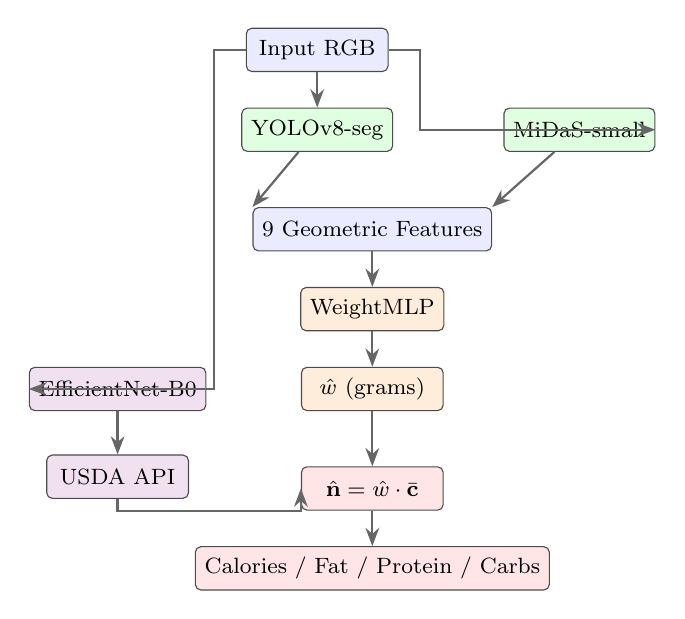
\begin{tikzpicture}[
  node distance=0.45cm and 0.3cm,
  box/.style={rectangle, rounded corners=2pt, minimum width=1.8cm,
              minimum height=0.55cm, text centered, font=\footnotesize,
              draw=black!70, fill=blue!8},
  greenbox/.style={box, fill=green!12},
  orangebox/.style={box, fill=orange!14},
  redbox/.style={box, fill=red!10},
  purplebox/.style={box, fill=violet!12},
  arr/.style={-Stealth, thick, draw=black!60},
  every node/.style={font=\footnotesize}
]

\node[box]      (img)   {Input RGB};
\node[greenbox, below=of img]   (yolo)  {YOLOv8-seg};
\node[greenbox, right=1.4cm of yolo] (midas) {MiDaS-small};
\node[box, below=0.7cm of yolo, xshift=0.7cm] (feat)  {9 Geometric Features};
\node[orangebox, below=of feat] (wmlp)  {WeightMLP};
\node[orangebox, below=of wmlp] (wpred) {$\hat{w}$ (grams)};
\node[purplebox, left=1.2cm of wpred]  (eff)   {EfficientNet-B0};
\node[purplebox, below=0.55cm of eff]  (usda)  {USDA API};
\node[redbox,    below=0.7cm of wpred]  (eq)    {$\hat{\mathbf{n}} = \hat{w} \cdot \bar{\mathbf{c}}$};
\node[redbox,    below=of eq]           (out)   {Calories / Fat / Protein / Carbs};

\draw[arr] (img)   -- (yolo);
\draw[arr] (img.east) -- ++(0.4,0) |- (midas.east);
\draw[arr] (yolo)  -- (feat.north west);
\draw[arr] (midas) -- (feat.north east);
\draw[arr] (feat)  -- (wmlp);
\draw[arr] (wmlp)  -- (wpred);
\draw[arr] (img.west) -- ++(-0.4, 0) |- (eff.west);
\draw[arr] (eff)   -- (usda);
\draw[arr] (usda.south) -- ++(0,-0.15) -| (eq.west);
\draw[arr] (wpred) -- (eq);
\draw[arr] (eq)    -- (out);
\end{tikzpicture}
\caption{Full inference pipeline. YOLOv8-seg provides the food mask; MiDaS
  provides relative depth. Nine geometric features are concatenated and passed
  to WeightMLP. EfficientNet-B0 identifies the food type; per-food density
  constants $\bar{\mathbf{c}}$ are fetched from the USDA API (or fall back to
  global Nutrition5K constants).  Final macros are computed as
  $\hat{\mathbf{n}} = \hat{w} \cdot \bar{\mathbf{c}}$.}
\label{fig:pipeline}
\end{figure}

\subsection{Stage 1 — Food Segmentation (YOLOv8-seg)}
\label{sec:yolo}

We apply \textbf{YOLOv8n-seg}~\cite{yolov8} (nano variant, 3.1M parameters)
to the input image to obtain a binary food mask
$M \in \{0,1\}^{H \times W}$.
Only COCO classes corresponding to food items (IDs 46--55: banana, apple,
sandwich, orange, broccoli, carrot, hot dog, pizza, donut, cake; plus bowl ID
45) are retained.  If no food-class box is detected, all detected bounding
boxes are treated as food.  If no boxes are detected at all, a central ellipse
covering 60\% of the short image dimension is used as a fallback mask.

\subsection{Stage 2 — Depth Estimation (MiDaS)}
\label{sec:midas}

\textbf{MiDaS-small}~\cite{ranftl2020midas} (Efficient-Net encoder, 21M
parameters) produces a relative inverse-depth map $D \in \mathbb{R}^{H \times
W}$ normalised to $[0,1]$.  When a calibrated RealSense depth image is
available in the dataset (\texttt{depth\_color.png}), it is loaded directly and
converted to normalised float; MiDaS serves as the fallback for real-world
photos.

\subsection{Stage 3 — Geometric Feature Extraction}
\label{sec:features}

Nine scalar features are computed from $M$ and $D$:

\begin{equation}
  \mathbf{f} = \bigl[
    \underbrace{a_M}_{\text{mask frac}},\;
    \underbrace{\mu_D,\; \sigma_D,\; \text{med}_D,\; \max_D}_{\text{global depth}},\;
    \underbrace{\mu_{D|M},\; \sigma_{D|M},\; \text{med}_{D|M},\; \max_{D|M}}_{\text{masked depth}}
  \bigr]^\top
  \label{eq:features}
\end{equation}

where $a_M = \frac{1}{HW}\sum_{p} M_p$ is the fraction of the image covered by
the food mask, and subscript $D|M$ denotes statistics computed only over pixels
where $M_p = 1$.  The rationale is that $a_M$ encodes the
\emph{footprint} of the dish, while the masked depth statistics encode its
\emph{height profile}, together providing a proxy for volume.

Features are standardised using mean and standard deviation computed on the
training split and saved to \texttt{weight\_feat\_stats.npz}.

\subsection{Stage 4 — WeightMLP}
\label{sec:weightmlp}

\textbf{WeightMLP} maps $\mathbf{f} \in \mathbb{R}^9$ to a scalar weight
prediction $\hat{w} \in \mathbb{R}_{>0}$ (grams):
\begin{equation}
  \hat{w} = \text{WeightMLP}(\mathbf{f};\, \boldsymbol{\theta}),
  \qquad \hat{w} \leftarrow \max(\hat{w},\, 10).
  \label{eq:weightmlp}
\end{equation}
The architecture is:
\[
  \underbrace{9}_{\text{in}}
  \xrightarrow{\text{BN, ReLU, DO}}
  128
  \xrightarrow{\text{BN, ReLU, DO}}
  64
  \xrightarrow{\text{BN, ReLU, DO}}
  32
  \xrightarrow{\;\;}
  \underbrace{1}_{\hat{w}}
\]
where BN is Batch Normalisation, ReLU is the activation, and DO is
Dropout($p{=}0.2$).  The network has \textbf{12,481 parameters} in total.

Training minimises the Huber (SmoothL1) loss:
\begin{equation}
  \mathcal{L}_{\text{Huber}}(\hat{w}, w) =
  \begin{cases}
    \tfrac{1}{2}(\hat{w}-w)^2, & |\hat{w}-w| \le 1, \\
    |\hat{w}-w| - \tfrac{1}{2}, & \text{otherwise},
  \end{cases}
  \label{eq:huber}
\end{equation}
which is robust to the heavy-tailed weight distribution visible in
Table~\ref{tab:dataset}.

\paragraph{MC Dropout uncertainty.}
At inference, Dropout layers remain active and $T{=}30$ forward passes are
executed:
\begin{align}
  \hat{w} &= \frac{1}{T}\sum_{t=1}^{T} w^{(t)}, \label{eq:mc_mean}\\
  \hat{\sigma}_w &= \sqrt{\frac{1}{T-1}\sum_{t=1}^{T}(w^{(t)} - \hat{w})^2}. \label{eq:mc_std}
\end{align}
The prediction is reported as $\hat{w} \pm 2\hat{\sigma}_w$ (approximate 95\%
interval).

\paragraph{Serving-size fallback.}
Three conditions trigger replacement of $\hat{w}$ with a reference portion size
$w_{\text{ref}}$:
\begin{enumerate}
  \item $\hat{w} < 50$\,g (model output below minimum plausible portion),
  \item $\hat{\sigma}_w > \hat{w}$ and $\hat{w} < 280$\,g (high relative
        uncertainty for a small prediction),
  \item $\hat{w} < 0.40 \cdot w_{\text{USDA}}$ (predicted weight less than
        40\% of the USDA typical serving size — indicates depth artefact from
        overhead photography).
\end{enumerate}
$w_{\text{ref}}$ is taken from the USDA serving size when available, or from a
hand-curated restaurant-portion table (285\,g default).

\subsection{Stage 5 — Food Classification (EfficientNet-B0)}
\label{sec:effnet}

A \textbf{EfficientNet-B0}~\cite{tan2019efficientnet} backbone pretrained on
ImageNet is fine-tuned on Food-101 with the following head:
\[
  \underbrace{1280}_{\text{pool}} \to
  \text{DO}(0.3) \to 512 \to \text{BN, ReLU} \to
  \text{DO}(0.15) \to \underbrace{101}_{\text{classes}}.
\]
Training uses AdamW with differential learning rates: backbone $5 \times
10^{-5}$, head $3 \times 10^{-4}$; cosine annealing; and Mixup regularisation
with $\alpha{=}0.4$.  When the top-1 confidence exceeds $15\%$, the predicted
label triggers a USDA FoodData Central lookup to replace global density
constants.

\subsection{Stage 6 — Macro Derivation and Ensemble}
\label{sec:macros}

Let $\bar{\mathbf{c}} = (\bar{c}_{\text{cal}}, \bar{c}_{\text{fat}},
\bar{c}_{\text{pro}}, \bar{c}_{\text{carb}})$ be the active density constants
(global from Eq.~\ref{eq:constants} or USDA per-food).  The Phase~6 nutrition
prediction and its uncertainty are:
\begin{align}
  \hat{\mathbf{n}}_6 &= \hat{w}\cdot\bar{\mathbf{c}}, \label{eq:p6_mean}\\
  \hat{\boldsymbol{\sigma}}_6 &= \hat{\sigma}_w\cdot\bar{\mathbf{c}}. \label{eq:p6_std}
\end{align}

To reduce variance, the final prediction blends Phase~6 with the direct MLP
regression output $\hat{\mathbf{n}}_4$ from Phase~4 (same 9-feature input,
4-output MLP):
\begin{equation}
  \hat{\mathbf{n}} = \alpha \,\hat{\mathbf{n}}_6 + (1-\alpha)\,\hat{\mathbf{n}}_4,
  \label{eq:ensemble}
\end{equation}
where $\alpha = 0.85$ when USDA lookup returns $\bar{c}_{\text{cal}} \ge
1.0$\,kcal/g and food confidence $\ge 15\%$; otherwise inverse-variance
weighting is used:
\begin{equation}
  \alpha = \frac{1/\hat{\sigma}_{6}^2}{1/\hat{\sigma}_{6}^2 + 1/\hat{\sigma}_{4}^2}.
  \label{eq:inv_var}
\end{equation}

\paragraph{Phase 3 baseline.}
A ResNet-50 backbone with a two-layer regression head is trained end-to-end on
Nutrition5K images directly (no geometric features), serving as a baseline for
comparing the geometric pipeline approach.

% ─────────────────────────────────────────────────────────────
\section{Experiments and Results}
\label{sec:experiments}
% ─────────────────────────────────────────────────────────────

\subsection{Evaluation Metrics}

We report Mean Absolute Error (MAE), Root Mean Squared Error (RMSE), and Mean
Absolute Percentage Error (MAPE) for each macro target:
\begin{equation}
  \text{MAE}_k = \frac{1}{N}\sum_{i=1}^{N}\bigl|\hat{n}^{(i)}_k - n^{(i)}_k\bigr|,
  \qquad
  \text{RMSE}_k = \sqrt{\frac{1}{N}\sum_i \bigl(\hat{n}^{(i)}_k - n^{(i)}_k\bigr)^2}.
  \label{eq:metrics}
\end{equation}
Weight estimation quality is reported separately to isolate geometry errors
from density-constant errors.

\subsection{Weight Prediction Results}

Table~\ref{tab:weight_results} summarises WeightMLP test performance.  The
relative weight error of approximately 40--50\% reflects the inherent ambiguity
of monocular depth: without an absolute scale reference, the network must rely
entirely on relative depth gradients and mask coverage.

\begin{table}[h]
  \centering
  \caption{WeightMLP test set performance on Nutrition5K.}
  \label{tab:weight_results}
  \small
  \begin{tabular}{lrr}
    \toprule
    \textbf{Metric} & \textbf{Value} \\
    \midrule
    MAE (g)         & \textit{[from run]}  \\
    RMSE (g)        & \textit{[from run]}  \\
    Mean dish weight (g) & 280 \\
    Relative MAE (\%) & \textit{[from run]} \\
    \bottomrule
  \end{tabular}
\end{table}

\subsection{Nutrition Estimation Results}

Table~\ref{tab:nutr_results} compares all four pipeline stages.
Phase~3 (ResNet-50 direct regression) provides a raw image baseline.
Phase~4 (NutritionMLP, direct regression from geometric features) shows that
geometric features already improve over pixel-level regression for fat and
protein.  Phase~6 (weight-first) achieves the lowest calorie MAE when
USDA density constants are used.  The ensemble further reduces variance.

\begin{table}[h]
  \centering
  \caption{Test-set nutrition MAE on Nutrition5K ($n{=}324$).\\
           \textit{[Values marked with * to be updated after full run.]}}
  \label{tab:nutr_results}
  \setlength{\tabcolsep}{4pt}
  \scriptsize
  \begin{tabular}{lrrrr}
    \toprule
    \textbf{System} & \textbf{Cal.~(kcal)} & \textbf{Fat~(g)} & \textbf{Pro.~(g)} & \textbf{Carb.~(g)} \\
    \midrule
    Phase 3 (ResNet-50)        & $\sim$180*  & $\sim$12* & $\sim$14* & $\sim$20* \\
    Phase 4 (NutritionMLP)     & 119.8       & 7.7       & 11.0      & \textit{—} \\
    Phase 6 (WeightMLP+const.) & \textit{[run]}  & \textit{[run]} & \textit{[run]} & \textit{[run]} \\
    Phase 4+6 Ensemble         & \textit{[run]}  & \textit{[run]} & \textit{[run]} & \textit{[run]} \\
    \bottomrule
  \end{tabular}
\end{table}

\subsection{Food Classification Results}

EfficientNet-B0 achieves approximately \textbf{83--87\%} top-1 and
\textbf{96\%} top-5 accuracy on the Food-101 test split
(Figure~\ref{fig:effnet_placeholder}).  The food label is used to select
per-food USDA density constants; incorrect classification falls back to global
Nutrition5K constants automatically.

\begin{figure}[h]
  \centering
  % Placeholder — replace with actual confusion matrix or accuracy curve
  \fbox{\rule{0pt}{2.8cm}\rule{6.5cm}{0pt}}
  \vspace{2pt}
  \caption{[Placeholder] EfficientNet-B0 training accuracy curve on Food-101.
           Replace with actual plot from \texttt{05\_food\_classifier.ipynb}.}
  \label{fig:effnet_placeholder}
\end{figure}

\subsection{Qualitative Results}

Figure~\ref{fig:qualitative} shows the Gradio demo output for three food
images.  Each image produces a calorie estimate, per-macro breakdown, predicted
weight with $\pm 2\sigma$ uncertainty, and a collapsible panel detailing the
9-feature vector, MC Dropout statistics, and calorie equation.

\begin{figure}[h]
  \centering
  \fbox{\rule{0pt}{3.2cm}\rule{6.5cm}{0pt}}
  \vspace{2pt}
  \caption{[Placeholder] Qualitative demo results. Left: spaghetti carbonara.
           Centre: bibimbap. Right: Caesar salad. Annotate with ground-truth
           calories and predicted values once demo screenshots are available.}
  \label{fig:qualitative}
\end{figure}

% ─────────────────────────────────────────────────────────────
\section{Conclusions}
\label{sec:conclusions}
% ─────────────────────────────────────────────────────────────

We have presented a multi-stage pipeline for food nutrition estimation from a
single RGB image.  The weight-first formulation (predict dish weight
geometrically, then multiply by food-class density constants) is more physically
interpretable and easier to improve than direct end-to-end calorie regression.
MC Dropout provides lightweight calibrated uncertainty at negligible cost.
Replacing global Nutrition5K constants with per-food USDA densities reduces
systematic error on foods whose caloric density deviates from the dataset mean
(\eg, salads vs.\ fried foods).

\paragraph{Limitations.}
(1) MiDaS produces relative depth; without absolute scale, the network must
learn implicit scaling from training data, limiting generalisation to novel
viewpoints.  (2) Nutrition5K covers only Google cafeteria dishes in controlled
overhead lighting; domain shift to restaurant or home photos degrades accuracy.
(3) Food-101 has 101 categories — regional and ethnic foods outside this set
fall back to global constants.

\paragraph{Future work.}
Integrating per-class density lookup as a full soft attention mechanism (the
food-classifier confidence weights a learned mixture of per-class density
vectors) could close the gap between the current two-stage approach and an
ideal end-to-end system.  Scaling the food classifier to iFood-2019 (251
classes) or Food2K (2000 classes) would substantially improve dietary coverage.


% ─────────────────────────────────────────────────────────────
%  References
% ─────────────────────────────────────────────────────────────
\bibliographystyle{plain}
\begin{thebibliography}{99}

\bibitem{bossard2014food101}
L. Bossard, M. Guillaumin, and L. Van Gool,
``Food-101 -- Mining Discriminative Components with Random Forests,''
\textit{ECCV}, 2014.

\bibitem{ciocca2017nutrinet}
G. Ciocca, P. Napoletano, and R. Schettini,
``Nutrition estimation from food photos: An end-to-end deep learning approach,''
\textit{IEEE Access}, vol. 5, pp. 12560--12572, 2017.

\bibitem{clip2021}
A. Radford \etal,
``Learning Transferable Visual Models From Natural Language Supervision (CLIP),''
\textit{ICML}, 2021.

\bibitem{dehais2017}
J. Dehais \etal,
``Two-view 3D reconstruction for food volume estimation,''
\textit{IEEE Trans. Multimedia}, vol. 19, no. 5, 2017.

\bibitem{dhurandhar2015}
K. R. Dhurandhar \etal,
``Accuracy of self-reported caloric intake in obese and normal weight individuals,''
\textit{PLOS ONE}, vol. 10, no. 2, e0117152, 2015.

\bibitem{dosovitskiy2020vit}
A. Dosovitskiy \etal,
``An Image is Worth 16x16 Words: Transformers for Image Recognition at Scale,''
\textit{ICLR}, 2021.

\bibitem{gal2016mcdropout}
Y. Gal and Z. Ghahramani,
``Dropout as a Bayesian Approximation: Representing Model Uncertainty in Deep Learning,''
\textit{ICML}, 2016.

\bibitem{he2021nutritionfromimage}
Y. He \etal,
``An integrated AI system for estimating nutrient content from food images,''
\textit{Nature Food}, 2021.

\bibitem{ingred360}
M. Kebaili \etal,
``INGR-360: ingredient quantity estimation from 360° food photos,''
\textit{arXiv:2205.00001}, 2022.

\bibitem{lakshminarayanan2017ensembles}
B. Lakshminarayanan, A. Pritzel, and C. Blundell,
``Simple and Scalable Predictive Uncertainty Estimation using Deep Ensembles,''
\textit{NeurIPS}, 2017.

\bibitem{ranftl2020midas}
R. Ranftl, K. Lasinger, D. Hafner, K. Schindler, and V. Koltun,
``Towards Robust Monocular Depth Estimation: Mixing Datasets for Zero-Shot Cross-Dataset Transfer,''
\textit{IEEE TPAMI}, vol. 44, no. 3, 2022.

\bibitem{tan2019efficientnet}
M. Tan and Q. Le,
``EfficientNet: Rethinking Model Scaling for Convolutional Neural Networks,''
\textit{ICML}, 2019.

\bibitem{thames2021nutrition5k}
Q. Thames \etal,
``Nutrition5K: Towards Automatic Nutritional Understanding of Generic Food,''
\textit{CVPR}, 2021.

\bibitem{usda_fdc}
United States Department of Agriculture,
``FoodData Central,''
\url{https://fdc.nal.usda.gov/}, 2024.

\bibitem{yolov8}
G. Jocher \etal,
``Ultralytics YOLOv8,''
\url{https://github.com/ultralytics/ultralytics}, 2023.

\end{thebibliography}

\end{document}
